\documentclass[lettersize,journal]{IEEEtran}
\usepackage{amsmath,amsfonts,amssymb}
\usepackage{algorithm}
\usepackage{algpseudocode}
\renewcommand{\Comment}[1]{\hfill$\triangleright$ #1}
\usepackage{array}
\usepackage{arydshln}
\usepackage{textcomp}
\usepackage{stfloats}
\usepackage{url}
\usepackage{graphicx}
\usepackage{tikz}
\usepackage{pgfplots}
\pgfplotsset{compat=1.17}
\usetikzlibrary{arrows.meta,positioning,shapes.geometric,calc}
\usepackage{hyperref}
\usepackage{xcolor}
\usepackage{setspace}
\hyphenation{op-tical net-works semi-conduc-tor IEEE-Xplore}
\usepackage{balance}
\setlength{\textfloatsep}{5pt}
\setlength{\floatsep}{4pt}
\setlength{\intextsep}{5pt}
\setlength{\abovecaptionskip}{3pt}
\setlength{\belowcaptionskip}{1pt}
\setlength{\abovedisplayskip}{3pt plus 1pt minus 1pt}
\setlength{\belowdisplayskip}{3pt plus 1pt minus 1pt}
\setlength{\abovedisplayshortskip}{1pt plus 1pt}
\setlength{\belowdisplayshortskip}{1pt plus 1pt}

\tikzset{
  veh/.style={circle, draw=black!70, fill=orange!35, minimum size=5mm, font=\small, line width=0.6pt},
  vehbad/.style={circle, draw=red!70!black, dashed, fill=orange!20, minimum size=5mm, font=\small, line width=0.9pt},
  ctrl/.style={rectangle, draw=black!70, fill=blue!12, minimum width=11mm, minimum height=5mm, font=\small, line width=0.6pt, rounded corners=1.2pt},
  ctrlbad/.style={rectangle, draw=red!70!black, fill=red!14, minimum width=11mm, minimum height=5mm, font=\small, line width=1.1pt, rounded corners=1.2pt},
  rsu/.style={rectangle, draw=black!70, fill=green!16, minimum width=7mm, minimum height=3.6mm, font=\small, line width=0.6pt, rounded corners=0.8pt},
  rsubad/.style={rectangle, draw=red!70!black, fill=red!16, minimum width=7mm, minimum height=3.6mm, font=\small, line width=1pt, rounded corners=0.8pt},
  atk/.style={regular polygon, regular polygon sides=3, draw=red!70!black, fill=red!25, minimum size=4mm, font=\small, line width=1pt},
  dataflow/.style={-{Latex[length=2mm,width=1.4mm]}, thick, blue!55!black, shorten >=1pt},
  ctrlflow/.style={-{Latex[length=2mm,width=1.4mm]}, dashed, green!45!black, line width=0.8pt, shorten >=1pt},
  hiddenflow/.style={-{Latex[length=2mm,width=1.4mm]}, dashed, red!65!black, line width=0.9pt, shorten >=1pt},
  stepnum/.style={circle, draw=black!80, fill=white, minimum size=3.4mm, font=\small, inner sep=0pt, line width=0.5pt},
  pktdelay/.style={rectangle, draw=red!70!black, fill=white, minimum width=2.2mm, minimum height=1.6mm, line width=0.8pt},
  pktfab/.style={rectangle, draw=red!70!black, fill=red!35, minimum width=2.2mm, minimum height=1.6mm},
  pktdup/.style={rectangle, draw=orange!80!black, fill=orange!35, minimum width=2.2mm, minimum height=1.6mm},
}
\newcommand{\floodicon}[1]{
  \node[rectangle, draw=orange!70!black, fill=orange!15, minimum width=2.1mm, minimum height=1.4mm, line width=0.5pt] at ($(#1)+(-0.07,-0.05)$) {};
  \node[rectangle, draw=orange!70!black, fill=orange!15, minimum width=2.1mm, minimum height=1.4mm, line width=0.5pt] at ($(#1)+(0,0)$) {};
  \node[rectangle, draw=orange!80!black, fill=orange!35, minimum width=2.1mm, minimum height=1.4mm, line width=0.6pt] at ($(#1)+(0.07,0.05)$) {};
}
\newcommand{\mobilitymark}[1]{
  \draw[-{Stealth[length=1.6mm,width=1.2mm]}, black!55, line width=0.6pt] ($(#1)+(0.62,0.0)$) -- ++(0.3,0);
  \node[font=\small, black!55] at ($(#1)+(0.78,0.2)$) {$s$};
}

\begin{document}
	\title{Hydra: A Plane-Differentiated Attack Class Unifying Selective Time Delay and Hidden Forwarding Under Controller-Compromise and Mobility Amplification in SDVNs}
	\author{
		\IEEEauthorblockN{Patikiri Arachchige Don Shehan Nilmantha Wijesekara, Siyagunakosgodage Apsari Udithara Fernando,Lankahaluge Nipuni Kaushalya Fernando,Pathiraja Mudiyanselage Sajani Chamindi Bandara Gunarathna}
		\thanks{P.A.D.S.N. Wijesekara (nilmantha@eie.ruh.ac.lk) is with the Dept. of Electrical and Information Engineering, Faculty of Engineering, University of Ruhuna, Galle 80000, Sri Lanka.}
	}
	\markboth{IEEE Networking Letters}{Wijesekara: Hydra Attack Class Against Software-Defined Vehicular Networks}

	\maketitle

	\begin{abstract}
	Selective time delay and hidden forwarding are treated in software defined vehicular network literature as separate attack families. We show both are drawn from one capability. A forwarding node carries an authorized contract of destination and deadline, and we prove a stealthy attack can violate exactly one term of this contract, never both, since a joint violation would produce the anomaly a consistency check already catches. This proof shows the eight documented variants form the complete set, with no ninth possible. Mobility and controller compromise amplify both contract terms through the same closed form mechanisms rather than separately.
	\end{abstract}

	\begin{IEEEkeywords}
		Software defined vehicular networks, control plane security, forwarding contract, controller compromise, mobility.
	\end{IEEEkeywords}

%% ================================================================
\section{Introduction}
%% ================================================================
\IEEEPARstart{A}{ny} flow a controller admits into an SDVN carries two promises: arrival by some deadline, and arrival nowhere outside an authorized destination set. OpenFlow does not separate these into two attackable objects, so it is worth asking why the literature does. Selective time delay work targets the deadline alone \cite{pascoal2017tap,sfto2023}; hidden forwarding work targets the destination alone \cite{fade2016,sdnsec2016}; controller compromise is studied only as an amplifier for whichever single family a paper is about \cite{wang2020topology}. None asks whether a covert break of either promise is drawn from one shared capability rather than two unrelated ones. A companion paper evaluates both families jointly under simultaneous attack \cite{nexus2026}, but as two surfaces needing two detectors, not one reducible object; each family's full formal treatment is given separately in \cite{phantom2026} and \cite{vanguardhf2026}.

This letter argues the two are one thing. A packet arriving late but unmodified at the right place is a deadline break alone; a packet whose copy reaches an unauthorized place while the original arrives on time and unaltered is a destination break alone. No documented variant ever breaks both at once, and this is not incidental but forced by covertness itself: breaking both promises together is precisely the anomaly a volumetric or consistency check is built to catch.

Five things are reported here for what we believe is the first time. First, a formal model reducing two previously unconnected attack families to two indicators over one packet level object. Second, a proof, from the covertness requirement rather than assumed, that the eight documented variants are complete and no ninth is possible. Third, closed form terms showing mobility and controller compromise amplify both indicators through the same two mechanisms, not separate, family specific ones. Fourth, an experiment design measuring this proposed threat model, both mechanisms active, against the same action with neither active, isolating each one's contribution. Fifth, each of Hydra's four data plane variants departs from how existing work models a compromised forwarding node in two connected ways: the acting entity need not hold any infrastructure position at all, since a compromised vehicle acting alone is already sufficient under the original attack model, and its opportunity is bounded to a recurring window that closes at every handoff, not the persistent, unbounded presence slow table exhaustion and forwarding anomaly work assumes for its own compromised switch.

%% ================================================================
\section{System and Adversary Model}
\label{sec:model}
%% ================================================================
\textit{Network Model:} Vehicles connect through a fixed grid of roadside units acting only as relays, while a flat, openly registered controller set makes every forwarding decision; no controller holds that role permanently, no roadside unit ever decides alone. Admitting packet class $p$ fixes a contract $\mathcal{K}(p) = \langle \mathcal{D}(p), \tau(p) \rangle$, an authorized destination set $\mathcal{D}(p)$ together with a delivery deadline $\tau(p)$, both checkable independently against the issuing controller's own committed record. A vehicle travels at speed $s$ and crosses roadside unit zones of radius $R$.

\textit{Adversary Model:} The adversary occupies exactly one plane at a time, never both from one actor: either a compromised controller issues instructions no roadside unit questions, or a compromised roadside unit or vehicle acts without waiting for any instruction. The adversary keeps within whatever budget a volumetric or consistency check would tolerate, so nothing it does looks wrong on its own. Once the controller itself is compromised, the mobility bounded window disappears entirely, since it already holds the zone's authoritative state and need not time anything against a vehicle's position.

%% ================================================================
\section{The Hydra Attack Class}
\label{sec:attack}
%% ================================================================
A breach is defined by what was delivered, not by what was intended. For packet $p$ delivered at time $t$ to destination $d$, the deadline indicator is given in Equation~\eqref{eq:chi-tau}.
\begin{equation}
\chi_\tau(p,t) = \mathbb{1}\!\left[t > \tau(p)\right]
\label{eq:chi-tau}
\end{equation}
In Equation~\eqref{eq:chi-tau}, $\chi_\tau$ equals one exactly when delivery misses its deadline, regardless of where the packet ended up. The destination indicator is given in Equation~\eqref{eq:chi-dest}.
\begin{equation}
\chi_D(p,d) = \mathbb{1}\!\left[d \notin \mathcal{D}(p)\right]
\label{eq:chi-dest}
\end{equation}
In Equation~\eqref{eq:chi-dest}, $\chi_D$ equals one exactly when some copy of $p$, whether the original or a duplicate, lands outside the authorized set, regardless of when it arrived.

\textit{Proposition.} Every stealthy variant satisfies exactly one of $\chi_\tau{=}1,\chi_D{=}0$ or $\chi_\tau{=}0,\chi_D{=}1$, and Table~\ref{tab:taxonomy} lists the complete set; no further stealthy variant exists beyond these eight. Suppose instead some variant broke both promises together, delivering a packet late and to an unauthorized destination in the same action. That action would trip a deadline check and disturb a destination or flow conservation check at once, which is exactly the compound anomaly such checks exist to catch, so no variant satisfying the stealth requirement can do this. Every documented variant is therefore confined to one side of the split. Under that constraint, three independent binary choices generate the whole space: which promise is broken, which plane the adversary sits at, and which of two mechanisms realizes the break at that plane, given in Equation~\eqref{eq:exhaustive}.
\begin{equation}
|\mathcal{V}| = \underbrace{2}_{\text{promise}} \times \underbrace{2}_{\text{plane}} \times \underbrace{2}_{\text{mechanism}} = 8
\label{eq:exhaustive}
\end{equation}
In Equation~\eqref{eq:exhaustive}, the mechanism pair takes a different concrete shape under each promise, direct delay against induced table exhaustion for $\chi_\tau$, fabrication against genuine retransmission for $\chi_D$, but the count is fixed once the stealth requirement rules out a fourth choice.

\begin{table}[t]
\centering
\caption{The Hydra Taxonomy}
\label{tab:taxonomy}
\footnotesize
\begin{tabular}{|c|c|c|c|}
\hline
\textbf{Var.} & \textbf{Plane} & \textbf{Promise} & \textbf{Mechanism} \\
\hline
S1 & Control & $\chi_\tau$ & Delaying flow modification \\
\hline
S2 & Data & $\chi_\tau$ & Direct packet buffering \\
\hline
S3 & Control & $\chi_\tau$ & Table saturating rule stream \\
\hline
S4 & Data & $\chi_\tau$ & Table flooding packet stream \\
\hline
S5 & Control & $\chi_D$ & Fabricated duplicate rule \\
\hline
S6 & Data & $\chi_D$ & Direct fabrication \\
\hline
S7 & Control & $\chi_D$ & Genuine copy reroute rule \\
\hline
S8 & Data & $\chi_D$ & Genuine passive retransmission \\
\hline
\end{tabular}
\end{table}

Fig.~\ref{fig:taxonomy} lays the eight variants out by plane, data plane on top and control plane directly below its matching pair, grouped by which promise and mechanism they belong to; the two rows share the same intent throughout and differ only in whether the compromised party acts on the data plane with its own hands or issues an instruction instead.
\begin{figure*}[t]
\centering
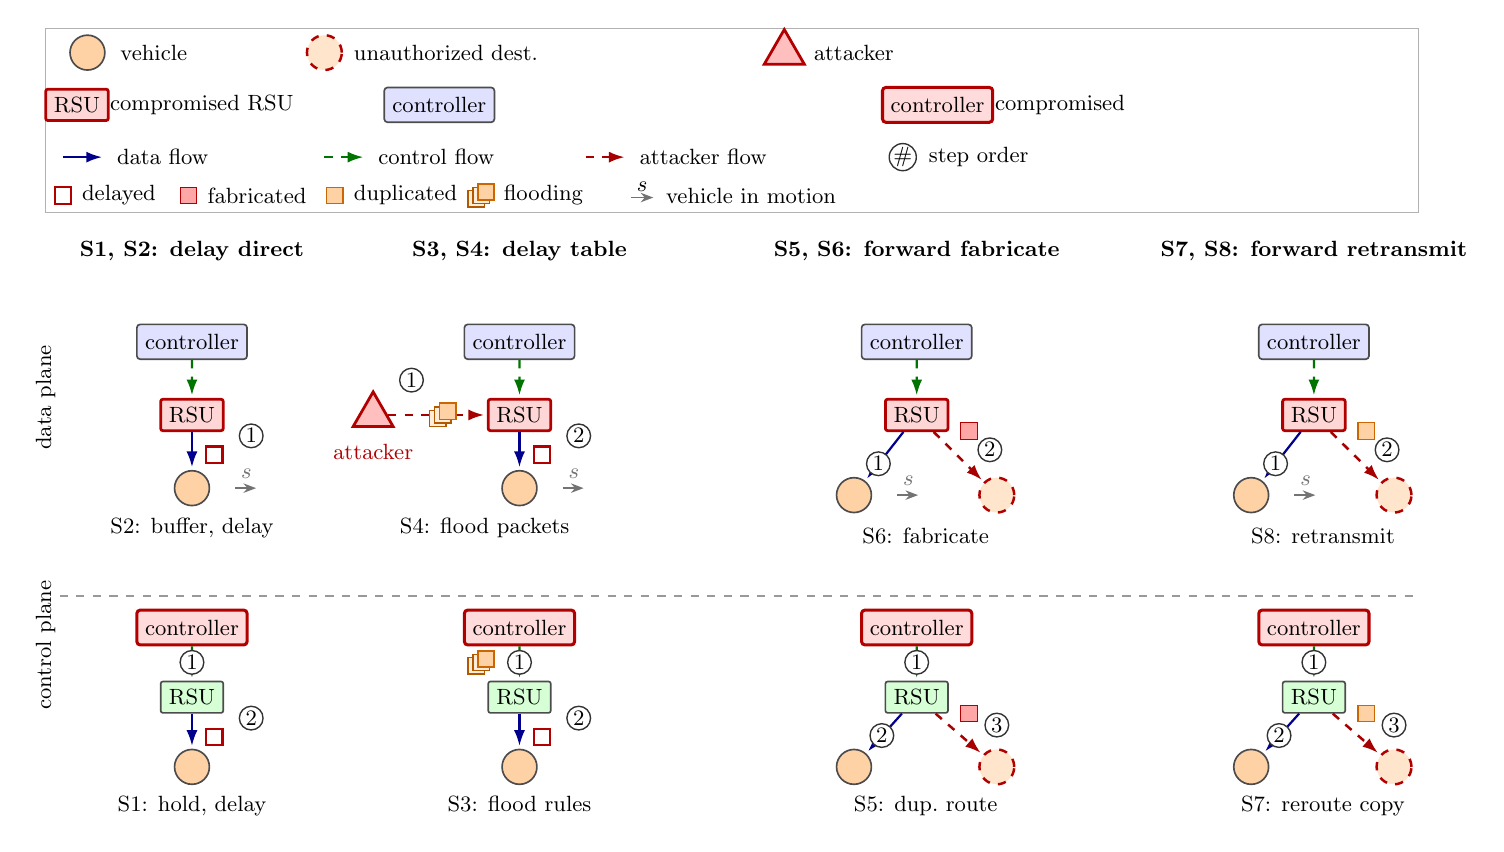
\begin{tikzpicture}[scale=0.885, transform shape, every node/.style={font=\normalsize}]

%% column centers, widened to 4.7 apart to accommodate generous internal spacing
%% col1=0, col2=4.7, col3=10.4, col4=16.1

\draw[draw=black!30] (-2.1,4.55) rectangle (17.6,7.2);
\begin{scope}[yshift=6.85cm]
\node[veh] at (-1.5,0) {};
\node[anchor=west,font=\small] at (-1.15,0) {vehicle};
\node[vehbad] at (1.9,0) {};
\node[anchor=west,font=\small] at (2.2,0) {unauthorized dest.};
\node[atk] at (8.5,0) {};
\node[anchor=west,font=\small] at (8.8,0) {attacker};
\end{scope}
\begin{scope}[yshift=6.1cm]
\node[rsubad] at (-1.65,0) {RSU};
\node[anchor=west,font=\small] at (-1.3,0) {compromised RSU};
\node[ctrl] at (3.55,0) {controller};
\node[ctrlbad] at (10.7,0) {controller};
\node[anchor=west,font=\small] at (11.4,0) {compromised};
\end{scope}
\begin{scope}[yshift=5.35cm]
\draw[dataflow] (-1.85,0) -- (-1.25,0); \node[anchor=west,font=\small] at (-1.2,0) {data flow};
\draw[ctrlflow] (1.9,0) -- (2.5,0); \node[anchor=west,font=\small] at (2.55,0) {control flow};
\draw[hiddenflow] (5.65,0) -- (6.25,0); \node[anchor=west,font=\small] at (6.3,0) {attacker flow};
\node[stepnum] at (10.2,0) {\#}; \node[anchor=west,font=\small] at (10.45,0) {step order};
\end{scope}
\begin{scope}[yshift=4.8cm]
\node[pktdelay] at (-1.85,0) {}; \node[anchor=west,font=\small] at (-1.7,0) {delayed};
\node[pktfab] at (-0.05,0) {}; \node[anchor=west,font=\small] at (0.1,0) {fabricated};
\node[pktdup] at (2.05,0) {}; \node[anchor=west,font=\small] at (2.2,0) {duplicated};
\floodicon{4.15,0}
\node[anchor=west,font=\small] at (4.35,0) {flooding};
\draw[-{Stealth[length=1.6mm,width=1.2mm]}, black!55, line width=0.6pt] (6.3,-0.03) -- (6.62,-0.03);
\node[font=\small] at (6.46,0.13) {$s$};
\node[anchor=west,font=\small] at (6.68,0) {vehicle in motion};
\end{scope}

\node at (0,4.0) {\textbf{\small S1, S2: delay direct}};
\node at (4.7,4.0) {\textbf{\small S3, S4: delay table}};
\node at (10.4,4.0) {\textbf{\small S5, S6: forward fabricate}};
\node at (16.1,4.0) {\textbf{\small S7, S8: forward retransmit}};
\node[rotate=90] at (-2.1,1.9) {\small data plane};
\node[rotate=90] at (-2.1,-1.65) {\small control plane};

%% ============ DATA PLANE ROW ============
\begin{scope}[xshift=0cm,yshift=0.8cm]
\node[ctrl] (c2) at (0,1.9) {controller};
\node[rsubad] (r2) at (0,0.85) {RSU};
\node[veh] (v2) at (0,-0.2) {};
\mobilitymark{v2}
\draw[ctrlflow] (c2) -- (r2);
\draw[dataflow] (r2) -- (v2);
\node[pktdelay] at (0.32,0.28) {};
\node[stepnum] at (0.85,0.55) {1};
\node[below,font=\small] at (0,-0.5) {S2: buffer, delay};
\end{scope}

\begin{scope}[xshift=4.7cm,yshift=0.8cm]
\node[ctrl] (c4) at (0,1.9) {controller};
\node[rsubad] (r4) at (0,0.85) {RSU};
\node[veh] (v4) at (0,-0.2) {};
\node[atk] (a4) at (-2.1,0.85) {};
\node[below,font=\small,red!70!black] at (-2.1,0.56) {attacker};
\mobilitymark{v4}
\draw[ctrlflow] (c4) -- (r4);
\draw[dataflow] (r4) -- (v4);
\draw[hiddenflow] (a4) -- (r4);
\floodicon{-1.1,0.85}
\node[stepnum] at (-1.55,1.35) {1};
\node[pktdelay] at (0.32,0.28) {};
\node[stepnum] at (0.85,0.55) {2};
\node[below,font=\small] at (-0.5,-0.5) {S4: flood packets};
\end{scope}

\begin{scope}[xshift=10.4cm,yshift=0.8cm]
\node[ctrl] (c6) at (0,1.9) {controller};
\node[rsubad] (r6) at (0,0.85) {RSU};
\node[veh] (v6) at (-0.9,-0.3) {};
\node[vehbad] (u6) at (1.15,-0.3) {};
\mobilitymark{v6}
\draw[ctrlflow] (c6) -- (r6);
\draw[dataflow] (r6) -- (v6);
\draw[hiddenflow] (r6) -- (u6);
\node[stepnum] at (-0.55,0.15) {1};
\node[stepnum] at (1.05,0.35) {2};
\node[pktfab] at (0.75,0.62) {};
\node[below,font=\small] at (0.13,-0.65) {S6: fabricate};
\end{scope}

\begin{scope}[xshift=16.1cm,yshift=0.8cm]
\node[ctrl] (c8) at (0,1.9) {controller};
\node[rsubad] (r8) at (0,0.85) {RSU};
\node[veh] (v8) at (-0.9,-0.3) {};
\node[vehbad] (u8) at (1.15,-0.3) {};
\mobilitymark{v8}
\draw[ctrlflow] (c8) -- (r8);
\draw[dataflow] (r8) -- (v8);
\draw[hiddenflow] (r8) -- (u8);
\node[stepnum] at (-0.55,0.15) {1};
\node[stepnum] at (1.05,0.35) {2};
\node[pktdup] at (0.75,0.62) {};
\node[below,font=\small] at (0.13,-0.65) {S8: retransmit};
\end{scope}

\draw[dashed,black!40,line width=0.6pt] (-1.9,-0.95) -- (17.6,-0.95);

%% ============ CONTROL PLANE ROW ============
\begin{scope}[xshift=0cm,yshift=-1.4cm]
\node[ctrlbad] (c1) at (0,0) {controller};
\node[rsu] (r1) at (0,-1.0) {RSU};
\node[veh] (v1) at (0,-2.0) {};
\draw[ctrlflow] (c1) -- (r1);
\draw[dataflow] (r1) -- (v1);
\node[stepnum] at (0,-0.5) {1};
\node[pktdelay] at (0.32,-1.57) {};
\node[stepnum] at (0.85,-1.3) {2};
\node[below,font=\small] at (0,-2.3) {S1: hold, delay};
\end{scope}

\begin{scope}[xshift=4.7cm,yshift=-1.4cm]
\node[ctrlbad] (c3) at (0,0) {controller};
\node[rsu] (r3) at (0,-1.0) {RSU};
\node[veh] (v3) at (0,-2.0) {};
\draw[ctrlflow] (c3) -- (r3);
\draw[dataflow] (r3) -- (v3);
\floodicon{-0.55,-0.5}
\node[stepnum] at (0,-0.5) {1};
\node[pktdelay] at (0.32,-1.57) {};
\node[stepnum] at (0.85,-1.3) {2};
\node[below,font=\small] at (0,-2.3) {S3: flood rules};
\end{scope}

\begin{scope}[xshift=10.4cm,yshift=-1.4cm]
\node[ctrlbad] (c5) at (0,0) {controller};
\node[rsu] (r5) at (0,-1.0) {RSU};
\node[veh] (v5) at (-0.9,-2.0) {};
\node[vehbad] (u5) at (1.15,-2.0) {};
\draw[ctrlflow] (c5) -- (r5);
\draw[dataflow] (r5) -- (v5);
\draw[hiddenflow] (r5) -- (u5);
\node[stepnum] at (0,-0.5) {1};
\node[stepnum] at (-0.5,-1.55) {2};
\node[stepnum] at (1.15,-1.4) {3};
\node[pktfab] at (0.75,-1.23) {};
\node[below,font=\small] at (0.13,-2.3) {S5: dup.\ route};
\end{scope}

\begin{scope}[xshift=16.1cm,yshift=-1.4cm]
\node[ctrlbad] (c7) at (0,0) {controller};
\node[rsu] (r7) at (0,-1.0) {RSU};
\node[veh] (v7) at (-0.9,-2.0) {};
\node[vehbad] (u7) at (1.15,-2.0) {};
\draw[ctrlflow] (c7) -- (r7);
\draw[dataflow] (r7) -- (v7);
\draw[hiddenflow] (r7) -- (u7);
\node[stepnum] at (0,-0.5) {1};
\node[stepnum] at (-0.5,-1.55) {2};
\node[stepnum] at (1.15,-1.4) {3};
\node[pktdup] at (0.75,-1.23) {};
\node[below,font=\small] at (0.13,-2.3) {S7: reroute copy};
\end{scope}

\end{tikzpicture}
\caption{Hydra attack variants.}
\label{fig:taxonomy}
\end{figure*}

Each variant asks for a different, specific capability. Among the four that break the deadline, S1 needs only the ability to issue a valid flow modification instructing the roadside unit to hold one targeted packet before release, while S3 turns that same ability into a stream of rules, pushed until the table starts missing legitimate lookups. Their data plane counterparts differ entirely: S2 needs direct standing on the forwarding path, buffering the packet with no controller instruction at all, and S4 needs only the ability to originate packets matching nothing installed, exhausting the same table by volume rather than command. Among the four that break the destination, S5 needs the ability to install a rule routing a second, fabricated copy alongside the original, and S6 carries out that same fabrication by hand at the node. S7 and S8 need less than fabrication, only the ability to hold a packet the actor already received honestly and release it later, so the copy reaching the unauthorized destination is genuinely signed. Fig.~\ref{fig:taxonomy} carries this distinction in its icon set: a compromised RSU for the data plane row, a compromised controller for the control plane row, and a motion arrow drawn only where an opportunity is mobility bounded.

Algorithm~\ref{alg:dataplane} carries out the four data plane variants under one procedure; the window it runs inside is not incidental, since a data plane actor never holds authoritative state and must act before the next handoff resets it. Algorithm~\ref{alg:ctrlplane} carries out the four control plane variants with no window at all, since a compromised controller already holds that state and races nothing.

The data plane variants also depart from how prior work models a compromised forwarding node. Slow table exhaustion and forwarding anomaly work treats that node as a fixed switch with an unbounded window, since its topology never changes \cite{pascoal2017tap,sfto2023,fade2016,sdnsec2016}. None of the four Hydra data plane variants admit such a persistent actor: whichever entity carries out S2, S4, S6, or S8 is confined to the window $\omega$ in Algorithm~\ref{alg:dataplane}, and need not hold any infrastructure position at all, since each of the four already permits an attacking vehicle acting alone, with no switch or controller access, a position the fixed switch models above do not admit as an attacker at all.

\begin{algorithm}[t]
\caption{Data Plane Procedure}
\label{alg:dataplane}
\begin{algorithmic}[1]
\small
\setstretch{0.9}
\Require variant $v\in\{\text{S2,S4,S6,S8}\}$, compromised node $n$ in zone $Z$, speed estimate $s$
\State compute residence window $\omega \gets 2R/s$
\While{within $\omega$ since entering $Z$, action not yet taken}
  \If{targeted packet $p$ observed at $n$}
    \If{$v=\text{S2}$}
      \State buffer $p$ for injected delay $A$; forward late \Comment{$\chi_\tau{=}1$}
    \ElsIf{$v=\text{S4}$}
      \State inject low rate uniquely matching packets toward table exhaustion \Comment{induces $\chi_\tau{=}1$}
    \ElsIf{$v=\text{S6}$}
      \State fabricate duplicate of $p$; forge signature; send to $d\notin\mathcal{D}(p)$ \Comment{$\chi_D{=}1$}
    \Else
      \State retransmit genuinely received $p$ to $d\notin\mathcal{D}(p)$ \Comment{$\chi_D{=}1$, signature valid}
    \EndIf
    \State \textbf{break}
  \EndIf
\EndWhile
\If{$\omega$ elapsed with no action taken}
  \State opportunity closes at handoff, unexecuted
\EndIf
\end{algorithmic}
\end{algorithm}

\begin{algorithm}[t]
\caption{Control Plane Procedure}
\label{alg:ctrlplane}
\begin{algorithmic}[1]
\small
\setstretch{0.9}
\Require variant $v\in\{\text{S1,S3,S5,S7}\}$, compromised controller $C$ of zone $Z$
\State $\mathcal{V} \gets$ flows currently assigned to $C$
\If{$v=\text{S1}$}
  \State issue FlowMod instructing RSU to hold targeted $p\in\mathcal{V}$ for $A$
\ElsIf{$v=\text{S3}$}
  \State issue low rate FlowMod stream driving RSU table toward saturation
\ElsIf{$v=\text{S5}$}
  \State issue FlowMod installing an unauthorized duplicate route for $p$
\Else
  \State issue FlowMod rerouting a genuine retransmission of $p$ to $d\notin\mathcal{D}(p)$
\EndIf
\State report nominal zone state upward
\end{algorithmic}
\end{algorithm}

%% ================================================================
\section{Analytical Model of Amplification}
\label{sec:analysis}
%% ================================================================
Both indicators are pushed by the same two mechanisms, mobility and controller compromise, rather than by anything specific to one family. How often a data plane opportunity comes around is given in Equation~\eqref{eq:handoff-rate}.
\begin{equation}
\lambda(s) = \frac{s}{L}
\label{eq:handoff-rate}
\end{equation}
In Equation~\eqref{eq:handoff-rate}, $L$ is the zone length, so $\lambda$ rises with speed, the formal reason opportunities recur more often at higher speed. How long any single opportunity lasts before the next handoff is given in Equation~\eqref{eq:dwell}.
\begin{equation}
\omega(s) = \frac{2R}{s}
\label{eq:dwell}
\end{equation}
In Equation~\eqref{eq:dwell}, $\omega$ falls as speed rises; the two equations describe the same handoff process from opposite sides, how often the window opens against how long it stays open.

An injected delay is only separable from ordinary handoff jitter where their densities pull apart, given in Equation~\eqref{eq:tau-overlap}.
\begin{equation}
\Psi(J,A) = -\ln\!\left(\int \sqrt{p_J(x)\,p_A(x)}\,dx\right)
\label{eq:tau-overlap}
\end{equation}
In Equation~\eqref{eq:tau-overlap}, $J$ is handoff jitter and $A$ the injected delay; $\Psi$ falls as handoff frequency climbs with speed, since the jitter density widens toward the injected one, with full derivation and measured thresholds in \cite{phantom2026}. Controller compromise removes this question outright, given in Equation~\eqref{eq:tau-gamma}.
\begin{equation}
\Phi_\tau = \frac{1}{1 - \Psi(J,A)/\Psi_{max}}
\label{eq:tau-gamma}
\end{equation}
In Equation~\eqref{eq:tau-gamma}, $\Phi_\tau$ grows without bound as $\Psi$ approaches $\Psi_{max}$, where mobility alone has erased any separation, and sits at one where mobility gives no cover, confirming the two mechanisms act independently on the same promise.

A duplicate can only be seen within the window a vehicle spends inside one zone, given in Equation~\eqref{eq:dest-window}.
\begin{equation}
\Omega(s) = \mu \cdot \omega(s)
\label{eq:dest-window}
\end{equation}
In Equation~\eqref{eq:dest-window}, $\mu$ is the sampling rate and $\Omega$ the samples one crossing offers, falling below whatever minimum a flow conservation check needs as speed rises, with the full statistical argument in \cite{vanguardhf2026}. Controller compromise removes this window the same way, given in Equation~\eqref{eq:dest-gamma}.
\begin{equation}
\Phi_D = \frac{\Omega_{min}}{\Omega(s)}
\label{eq:dest-gamma}
\end{equation}
In Equation~\eqref{eq:dest-gamma}, $\Phi_D$ exceeds one once mobility alone pushes the sample count below the minimum $\Omega_{min}$ required, and once the controller is compromised the check is moot regardless of $\Phi_D$, the same qualitative jump Equation~\eqref{eq:tau-gamma} shows for the deadline side.

Neither amplification term cares which mechanism realizes the underlying break, so one severity measure can weigh both promises without reference to variant identity, given in Equation~\eqref{eq:severity}.
\begin{equation}
\Sigma(s) = w_\tau\, \Phi_\tau(s) + w_D\, \Phi_D(s)
\label{eq:severity}
\end{equation}
In Equation~\eqref{eq:severity}, the weights $w_\tau,w_D$ let a deployment decide which promise matters more for a given service class, and $\Sigma$ climbs with speed under either choice, since $\Phi_\tau$ and $\Phi_D$ both do so alone.

%% ================================================================
\section{Attack Effectiveness Experiment}
\label{sec:experiment}
%% ================================================================
An NS-3 and SUMO simulation activates all eight variants together, splitting the targeted flow share evenly at attack percentage $p\in\{0,20,40,60,80,100\}\%$ across four configurations: neither mechanism, which stands in for how the cited literature already characterizes this same underlying action; mobility only; compromise only; and both together, matching this letter's own adversary model. Speed is held at a low, representative value under the two mobility off configurations and raised to a high one wherever mobility is active, isolating the speed dependence Equations~\eqref{eq:tau-overlap} through~\eqref{eq:dest-gamma} predict from the percentage sweep itself, rather than leaving speed implicit. Network scale, the roadside unit grid, and cryptographic parameters match the companion papers. The reported quantity, plotted in Fig.~\ref{fig:experiment}, is a pooled breach rate, the share of targeted packets whose relevant promise, deadline for the four $\chi_\tau$ variants and destination for the four $\chi_D$ variants, was actually broken; results are pending.

\begin{figure}[t]
\centering
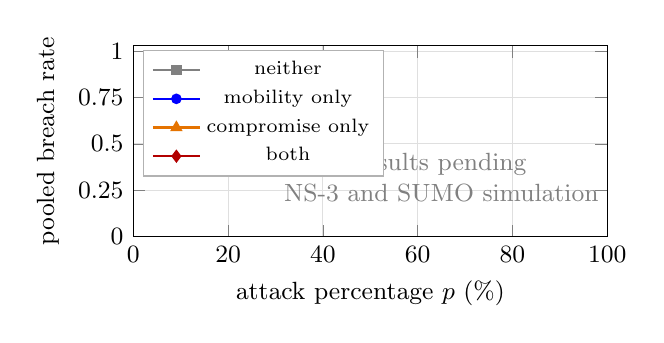
\begin{tikzpicture}
\begin{axis}[
  width=7.6cm,height=4.0cm,
  xlabel={attack percentage $p$ (\%)}, ylabel={pooled breach rate},
  xmin=0,xmax=100, ymin=0,ymax=1.03,
  xtick={0,20,40,60,80,100}, ytick={0,0.25,0.5,0.75,1},
  tick label style={font=\small}, label style={font=\small},
  legend style={font=\scriptsize,at={(0.02,0.98)},anchor=north west,draw=black!30},
  grid=major, grid style={gray!25},
]
\addlegendimage{thick,black!50,mark=square*,mark size=1.5pt}
\addlegendentry{neither}
\addlegendimage{thick,blue,mark=*,mark size=1.5pt}
\addlegendentry{mobility only}
\addlegendimage{thick,orange!90!black,mark=triangle*,mark size=1.8pt}
\addlegendentry{compromise only}
\addlegendimage{thick,red!70!black,mark=diamond*,mark size=1.8pt}
\addlegendentry{both}
\node[align=center,font=\small,black!50] at (axis cs:65,0.32) {results pending\\NS-3 and SUMO simulation};
\end{axis}
\end{tikzpicture}
\caption{Attack effectiveness.}
\label{fig:experiment}
\end{figure}

Mobility only is expected to exceed the neither configuration at every $p$, since Equations~\eqref{eq:tau-overlap} through~\eqref{eq:dest-gamma} predict both promises grow easier to break as speed narrows either window, and compromise only is expected to exceed mobility only in turn, since the adversary model removes that window rather than merely narrowing it. Both together is expected to dominate throughout, the direct empirical test of this letter's own proposed threat model against the same action taken with neither mechanism engaged. The pooled curve is expected to rise smoothly rather than in eight visible steps, since the eight variants share only two underlying promises between them, so any one configuration's effect on $\chi_\tau$ or $\chi_D$ shows up the same way regardless of which of the four variants realizing that promise is active.

%% ================================================================
\section{Security Analysis}
\label{sec:security}
%% ================================================================
Four properties hold across the whole class. Nothing here breaks authentication, since every action in Table~\ref{tab:taxonomy} is a legitimate protocol operation carried out under its own actor's real credentials. Nothing here breaks content integrity either, since $\chi_\tau$ variants deliver the packet unchanged and $\chi_D$ variants deliver a copy that is either unchanged or genuinely re signed. The Proposition of Section~\ref{sec:attack} carries a direct consequence for detection reach: a monitor built to watch one promise cannot see a break of the other, so a deadline check misses every $\chi_D$ variant by construction and a destination check misses every $\chi_\tau$ variant the same way. And the plane split carries its own blind spot, independent of which promise is at stake: a monitor stationed only on the data plane, watching how a roadside unit or vehicle actually forwards, never observes the instruction a compromised controller issued, so S1, S3, S5, and S7 leave no trace where such a monitor is looking, and a monitor stationed only on the control plane misses S2, S4, S6, and S8 the same way, since nothing about those four ever touches a flow modification at all.

%% ================================================================
\section{Conclusion}
%% ================================================================
This letter reported Hydra. Selective time delay and hidden forwarding, so far studied apart, are shown to break exactly one term of a two part forwarding contract, deadline or destination, at exactly one plane, and this letter proves that three binary choices account for the whole space, so the eight known variants are complete and no ninth is possible. Mobility and controller compromise are shown to push both promises through the same closed form terms, so selective time delay and hidden forwarding, each amplified on its own terms in prior work, are shown here to answer to one shared amplification model rather than two. Formal detection for each promise belongs to the companion papers \cite{phantom2026,vanguardhf2026}, with joint evaluation under simultaneous attack in \cite{nexus2026}; this letter's own contribution is the proof and the taxonomy it generates, not a new defense.

\section*{Acknowledgment}
None.

\balance
\begin{thebibliography}{10}
\footnotesize
\setlength{\itemsep}{0pt}
\setlength{\parsep}{0pt}
\setlength{\parskip}{0pt}
\bibitem{pascoal2017tap} T.~A. Pascoal, Y.~G. Dantas, I.~E. Fonseca, and V. Nigam, ``Slow TCAM exhaustion DDoS attack,'' in \textit{Proc. 32nd IFIP Int. Conf. ICT Syst. Secur. Privacy Prot. (IFIP SEC)}, Rome, Italy, 2017, pp. 17--31.
\bibitem{sfto2023} D. Tang, W. Zhang, \textit{et al.}, ``SFTO Guard: real time detection and mitigation system for slow rate flow table overflow attacks,'' \textit{J. Netw. Comput. Appl.}, 2023.
\bibitem{fade2016} C. Pang, Y. Jiang, and Q. Li, ``FADE: detecting forwarding anomaly in software defined networks,'' in \textit{Proc. IEEE Int. Conf. Commun. (ICC)}, 2016.
\bibitem{sdnsec2016} T. Sasaki, C. Pappas, T. Lee, T. Hoefler, and A. Perrig, ``SDNsec: forwarding accountability for the SDN data plane,'' in \textit{Proc. 25th Int. Conf. Comput. Commun. Netw. (ICCCN)}, IEEE, 2016, pp. 1--10.
\bibitem{wang2020topology} J. Wang, Y. Tan, J. Liu, and Y. Zhang, ``Topology poisoning attack in SDN-enabled vehicular edge network,'' \textit{IEEE Internet Things J.}, vol. 7, no. 10, pp. 9563--9574, 2020.
\bibitem{sedjelmaci2014} H. Sedjelmaci, S.~M. Senouci, and M.~A. Abu-Rgheff, ``An efficient and lightweight intrusion detection mechanism for service-oriented vehicular networks,'' \textit{IEEE Internet Things J.}, vol. 1, no. 6, pp. 570--577, 2014.
\bibitem{pukelsheim1994three} F. Pukelsheim, ``The three sigma rule,'' \textit{Amer. Statist.}, vol. 48, no. 2, pp. 88--91, 1994.
\bibitem{phantom2026} P.A.D.S.N. Wijesekara \textit{et al.}, ``PHANTOM: Mobility-adaptive, controller-inclusive zero-trust detection of selective time delay attacks in SDVN,'' under review, 2026.
\bibitem{vanguardhf2026} P.A.D.S.N. Wijesekara \textit{et al.}, ``VANGUARD-HF: Dual-mode detection of hidden forwarding attacks in SDVN,'' under review, 2026.
\bibitem{nexus2026} P.A.D.S.N. Wijesekara \textit{et al.}, ``NEXUS: Joint detection of selective time delay and hidden forwarding attacks in SDVN,'' under review, 2026.
\end{thebibliography}

\end{document}